\documentclass{article}
% set up the page formatting
\usepackage[a4paper, portrait, margin=2.5cm]{geometry}
\usepackage{multicol}
\usepackage{fancyhdr}
\usepackage{xcolor}
\usepackage{graphicx}
\usepackage{float}

% allow for table of contents clickable links
\usepackage{hyperref}

% editable bits
\title{CS261 Group 29 Planning and Design}
\author{Ani Bitri, Krister Hughes, Thomas Phuong, Eshan Sharif, Josh Turner, Antoni Zyla}
\date{January 2025}
\fancyfoot[L]{Planning and Design}
\fancyfoot[R]{\thepage}

\begin{document}
\maketitle
\tableofcontents

\section{Team Planning}
\subsection{Time Management}
In our meetings we have discussed how we are going to manage our time and have agreed to the following deadlines:

Below is a Gantt chart of our planned work schedule.

\begin{figure}[h!]
    \centering
    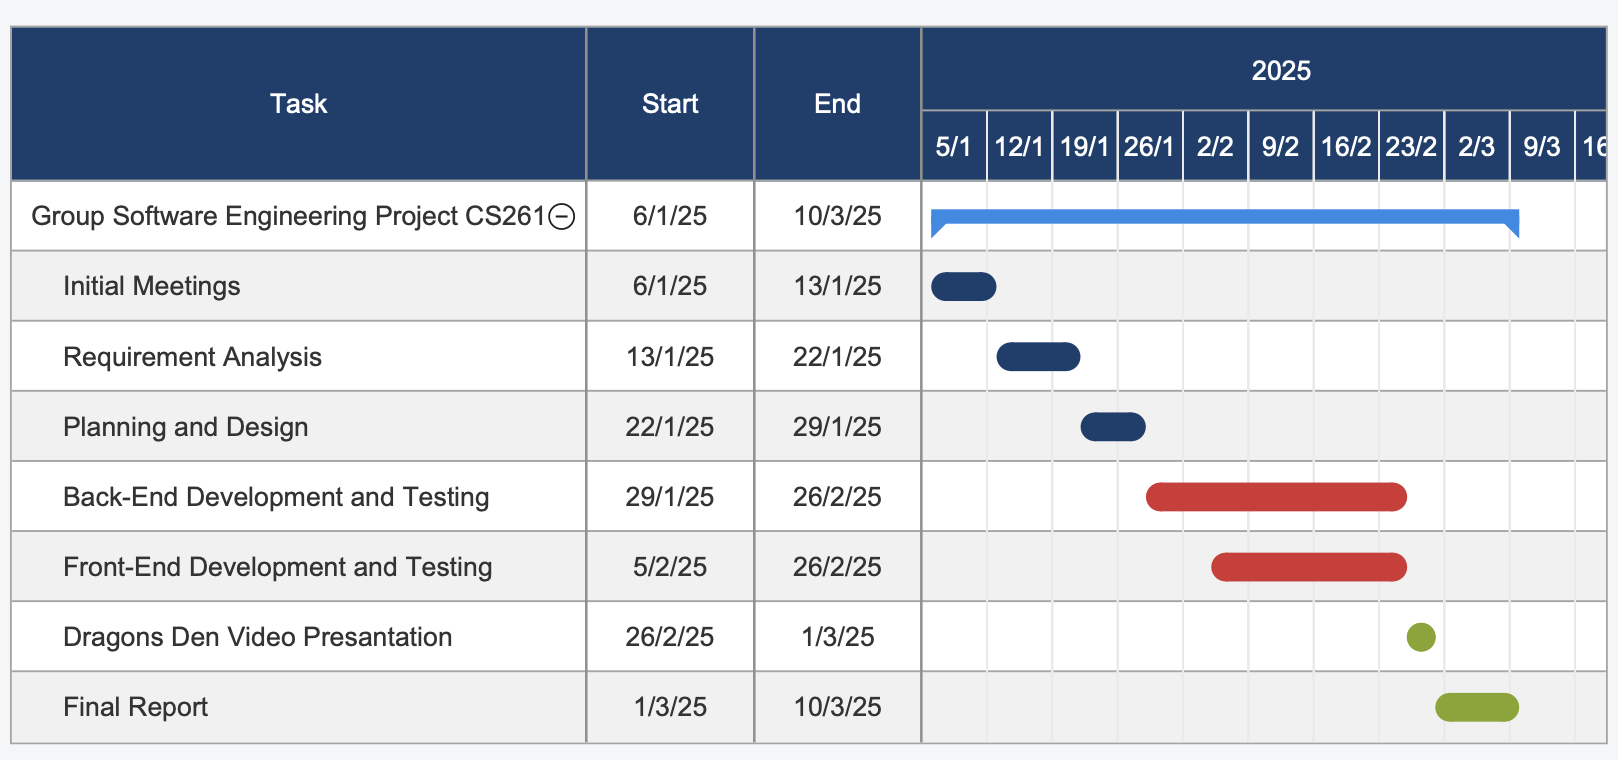
\includegraphics[width=\textwidth]{ganttchart.png}
    \caption{Gantt Chart of Planned Work Schedule}
    \label{fig:gantt_chart}
\end{figure}


\subsection{Risk Assessment and Management}
We have identified the following risks and have agreed on the following mitigation strategies:
\subsubsection{Technology Limitations}
\begin{itemize}
    \item Risk description: Team/Team members may be unfamiliar to some tool, libraries, or frameworks, which may cause delays or reduced performance. 
    \item Risk Level: \textcolor{green}{Tolerable}
    \item Risk Likelihood: \textcolor{orange}{Moderate}
    \item Mitigation Strategy: Assign tasks to team members based on their expertise in relevant technologies while ensuring everyone is involved in meaningful roles to maintain prductivity and foster teamwork.
\end{itemize}

\subsubsection{Rollback Challenges}
\begin{itemize}
    \item Risk description: Lack of a version control system could prevent from rolling back to the software's last stable state in case of errors
    \item Risk Level: \textcolor{red}{Catastrophic}
    \item Risk Likelihood: \textcolor{green}{Low}
    \item Mitigation Strategy: Utilise github to always maintain a stable version of the software and updating it when being sure that the changes will not affect its usability. 
\end{itemize}

\subsubsection{Testing Risks}
\begin{itemize}
    \item Risk description: Insufficient testing may reduce confidence in the software
    \item Risk Level: \textcolor{orange}{Serious}
    \item Risk Likelihood: \textcolor{orange}{Moderate}
    \item Mitigation Strategy: Unit tests will be designed to test the software to make sure that it is working properly.
\end{itemize}

\subsubsection{Time Management}
\begin{itemize}
    \item Risk description: Underestimating  task duration or improper prioritization might result in delayed work.
    \item Risk Level: \textcolor{orange}{Serious}
    \item Risk Likelihood: \textcolor{green}{Low}
    \item Mitigation Strategy: The team is meeting in regular intervals to ensure work efficiency and mitigate time related risks.
\end{itemize}

\subsubsection{Requirement Misalignment}
\begin{itemize}
    \item Risk description: During the development of the software, the end product might not be the same as the one describe in the deliverables due to unforeseen circumstances
    \item Risk Level: \textcolor{red}{Catastrophic}
    \item Risk Likelihood: \textcolor{green}{Low}
    \item Mitigation Strategy: Ensure constant internal communication between the team.
\end{itemize}

\subsubsection{Organisational Risks}
\begin{itemize}
    \item Risk description: Uneven distribution of workload or miscommunication may lead to an incomplete project and delayed work. 
    \item Risk Level: \textcolor{orange}{Serious}
    \item Risk Likelihood: \textcolor{green}{Low}
    \item Mitigation Strategy: The team is meeting in regular intervals to ensure work efficiency and mitigate time related risks.
\end{itemize}

\subsubsection{Team Member MIA}
\begin{itemize}
    \item Risk description: Team member is not able to complete their amount of work due to unforeseen circumstances, thus delaying work. 
    \item Risk Level: \textcolor{orange}{Serious}
    \item Risk Likelihood: \textcolor{orange}{Moderate}
    \item Mitigation Strategy: Team analyses the remaining work from missing member and prioritises and reallocates tasks based on the analysis. 
\end{itemize}

\section{Design Pattern}
We have decided to adopt the MVC (Model-View-Controller) design pattern for the software. This pattern consists of thre main components: the Model, the View and the Controller.
The Model is responsible for the data and the logic of the software, thus it will be our back-end. The View is responsible for the user interface and will be our front-end. The Controller is responsible for the communication between the Model and the View, 
thus it will be the API that we will use to interface between the front-end and back-end. The image beloww shows the MVC design pattern:

\begin{figure}[H]
    \centering
    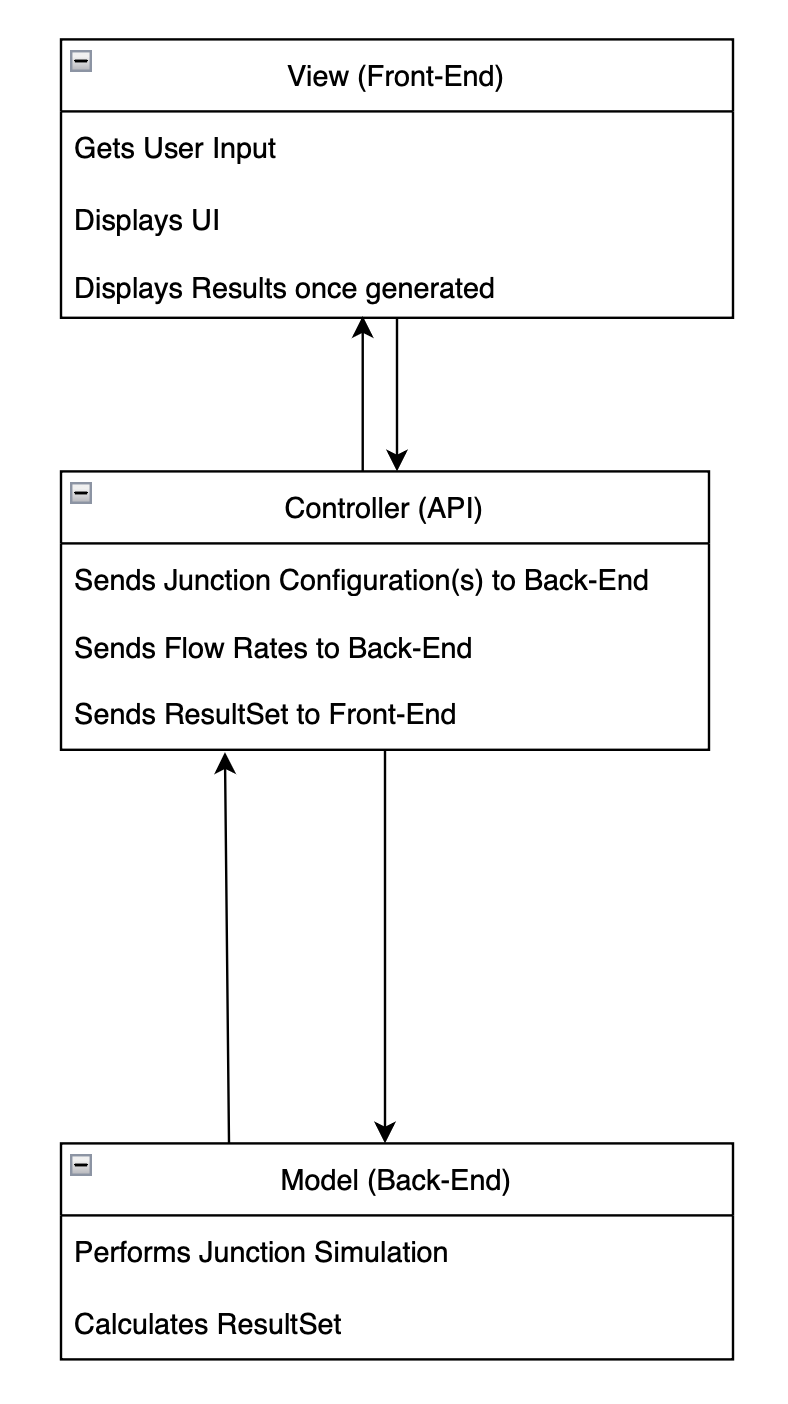
\includegraphics[width=0.5\textwidth]{pattern.png}
    \caption{MVC Pattern}
    \label{pattern}
\end{figure}

Using the MVC pattern will aid us in separating concerns, making the software more modular and easier to maintain. It will also help us separate the development responsibilities between the team members, with some working on the front-end, some on the back-end and some on the API.

\section{Front-End}
%Discussion of using Python and Pygame/similar libraries to create the user interface (including parsing user input) and graphics
For the front-end, we have decided to use Python and the PyQT toolkit to create the user interface. This is because the whole group is familiar 
with the frameworks, and it is a powerful and flexible toolkit that will allow us to create a user-friendly interface.

\subsection{User Interface}
The user interface will be designed to be simple and intuitive, with the user able to input the parameters of the junction configuration.
The picture below shows a mock-up of the user interface:

\begin{figure}[H]
    \centering
    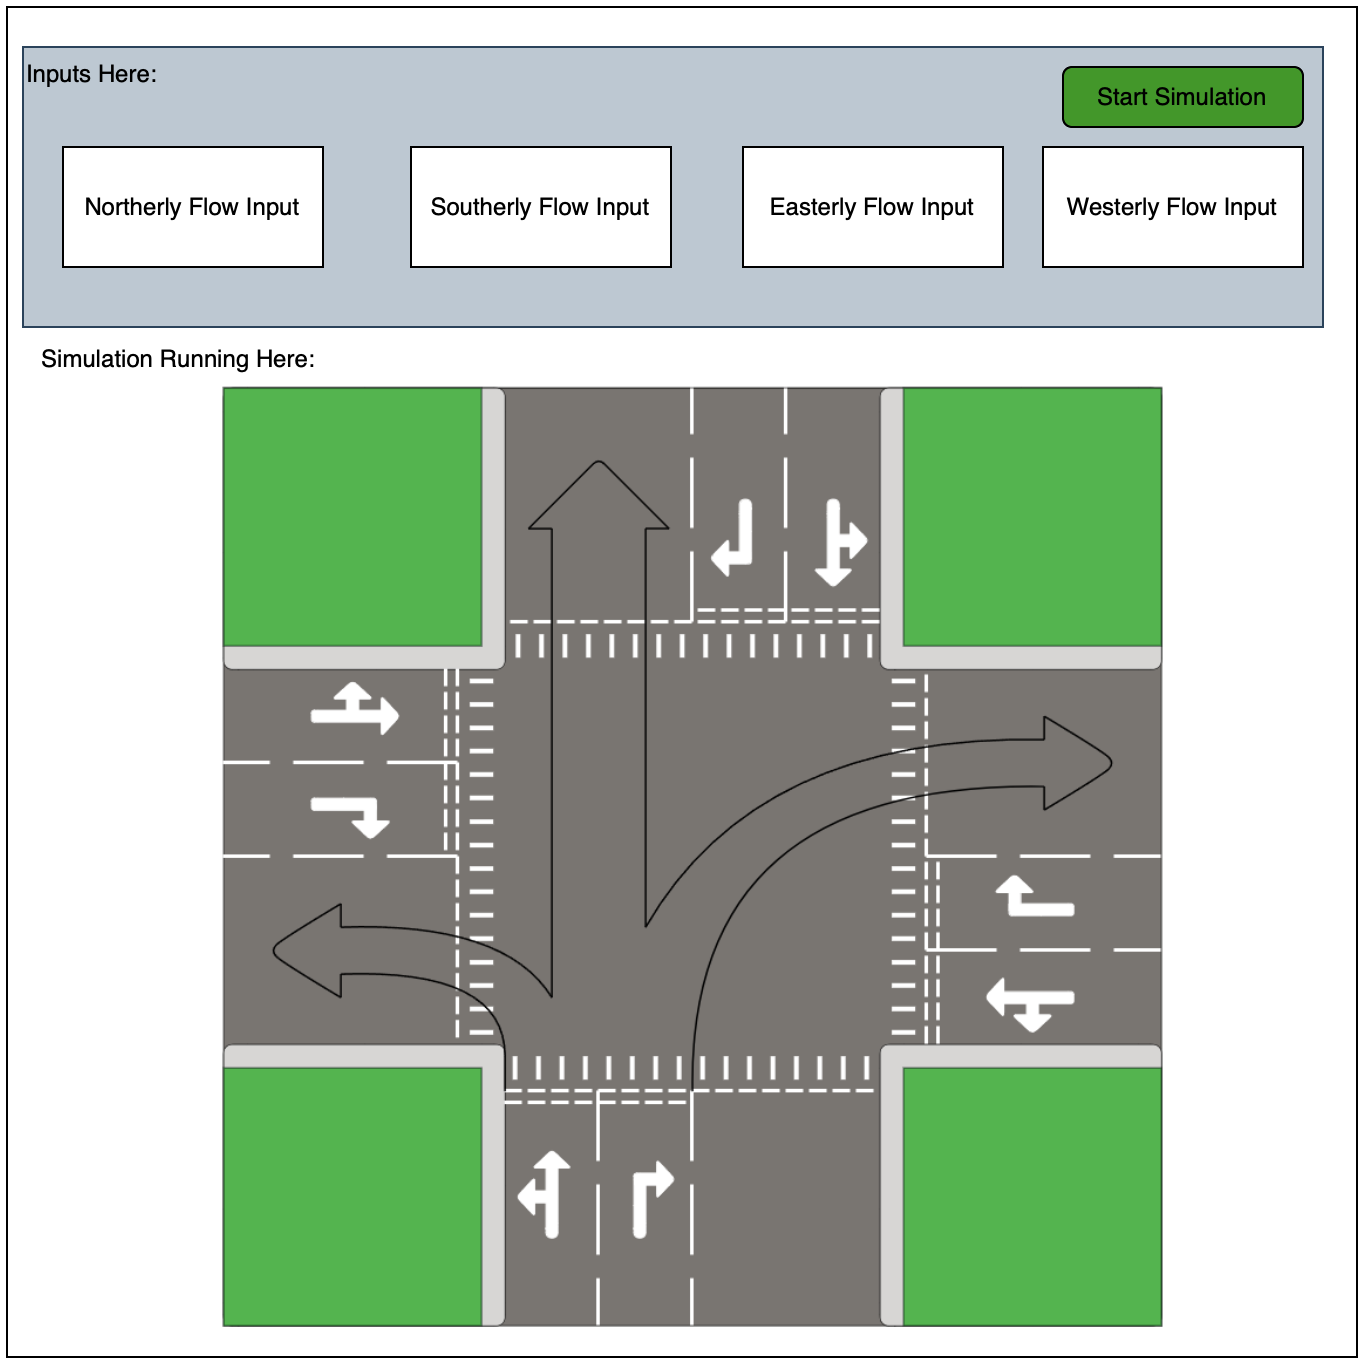
\includegraphics[width=0.8\textwidth]{frontendUI.png}
    \caption{Mock-up of the User Interface}
    \label{frontendUI}
\end{figure}

The user will be able to input the number of lanes on each road, the flow rates from each direction to the other directions and specific lanes such
as the bus lane, left-turn lane or right-turn lane. The simulation can start by clicking the "Start Simulation" button. The simulation will then run and the results will be displayed on the screen on a tabular format.
The figure below shows a mock-up of the results table:

\begin{figure}[H]
    \centering
    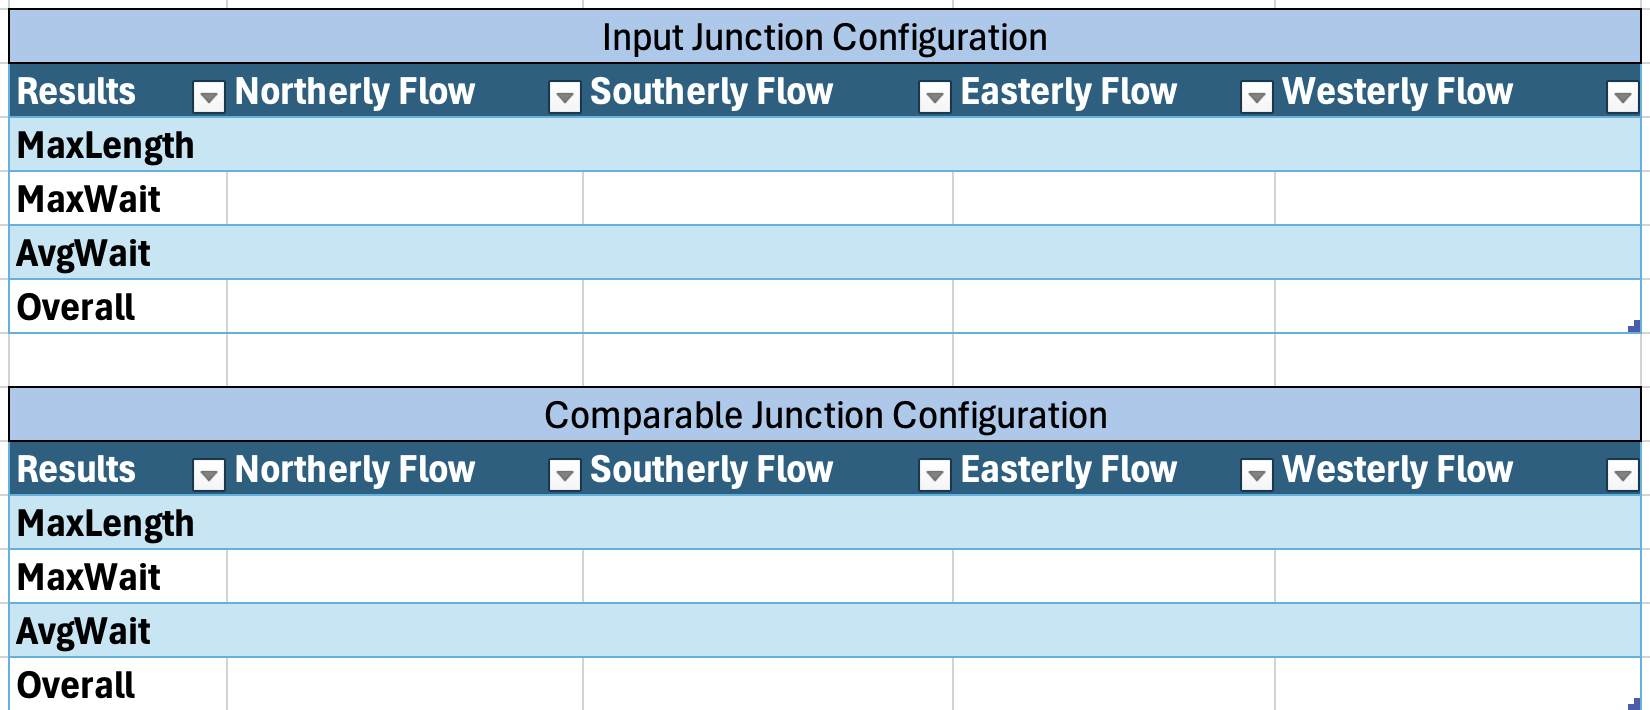
\includegraphics[width=0.8\textwidth]{frontendoutput.png}
    \caption{Mock-up of the Results Table}
    \label{frontendoutput}
\end{figure}

\subsection{Interfacing with Back-End}
Before accepting any user input, the front-end will validate the input to ensure that it is within the required range and that there are no conflicts between certain parameters.
The front-end will then pass the input to the back-end using an API. The back-end will run the simulation when the "Start Simulation" button is clicked and return the results to the front-end when the simulation finishes,
which will display them on the screen as described above.

\subsection{Error Handling}
Throughout the whole process of the software, from inputting the parameters to displaying the results, the front-end will have error handling to ensure that the software is robust and reliable.
Friendly error messages will be displayed to the user if they input invalid parameters or if there is an error in the simulation. The following pictures show examples of error messages that will be displayed:

\begin{figure}[H]
    \centering
    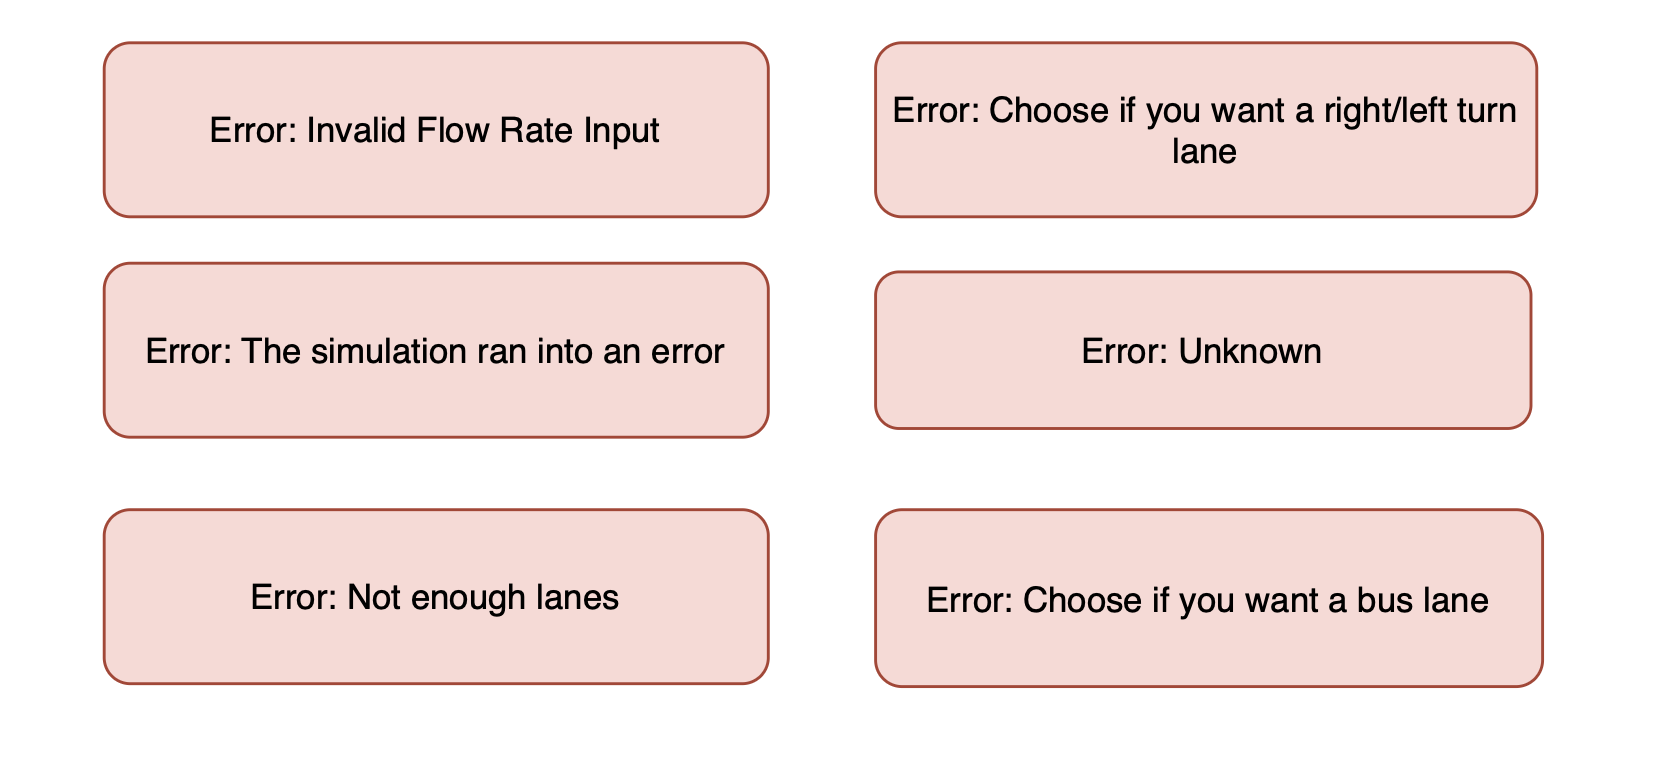
\includegraphics[width=\textwidth]{errormsg.png}
    \caption{Examples of Error Messages}
    \label{errormsg}
\end{figure}

\section{Back-End}
%Discussion of the design of the simulation
For the back-end, we have decided to implement it in Python due to the whole group being familiar with the language, and to make 
interfacing between the front-end and back-end simple. 

\subsection{Simulation}

We plan to use objects to simulate the junction configurations and calculate 
the junction efficiency metrics and overall scores, with the structure of classes being as follows:

\begin{figure}[H]
    \centering
    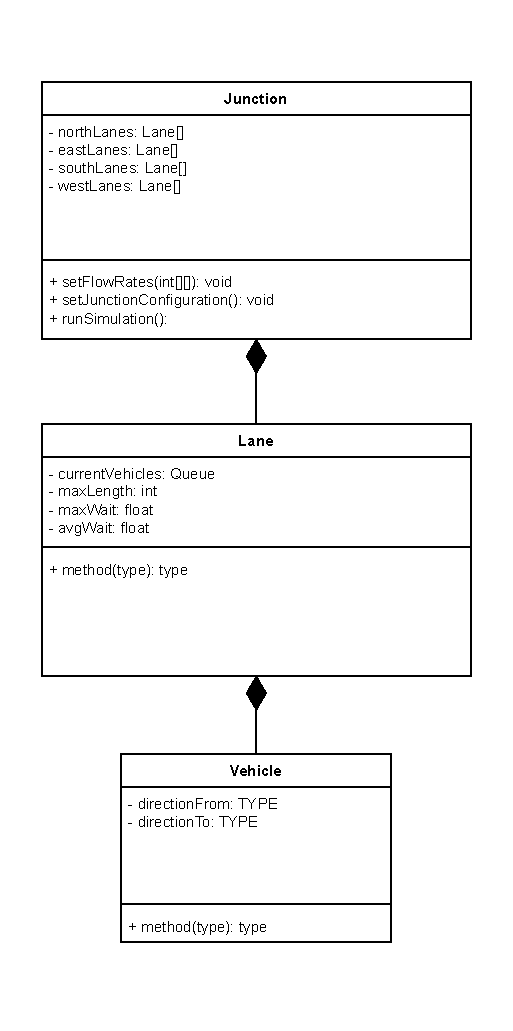
\includegraphics[width=0.8\textwidth]{JunctionSimulationClassDiagram.drawio.pdf}
    \caption{Junction Simulation Class Diagram}
    \label{class diagram}
\end{figure}

The Junction class contains Lane objects representing each lane of a road entering the junction, grouped together in arrays based on 
the direction they are arriving at the junction from. Two functions will be called by the front-end to set up the simulation: `setFlowRates` 
to set the flow rates from each direction to the other directions, passed in the form of a `FlowRates` object, and `setJunctionConfiguration` 
to set the specific settings of the junction (e.g. is there a left turn lane, how many lanes there are on each incoming road) passed in 
the form of a Parameters object. For each junction configuration generated by the user, a Junction object will be created and be passed 
a Parameters object corresponding to those configuration settings. We decided to use objects for passing the data instead of passing each 
setting as an individual parameter (`setJunctionConfiguration`) or passing the flow rates as a 2D-array (`setFlowRates`) since objects would 
be easier to work with (for example, no scope for miscommunication about what the indices represent) and make it easier to extend the 
capabilities of the software in the future.

Each Lane object contains a queue of Vehicle objects, representing the vehicles in that lane waiting to transit the junction. Each Lane 
will calculate its own maximum wait time (`maxWait`), average wait time (`avgWait`) and maximum queue length (`maxLength`), which will be 
compared with the same values of the other Lanes in its direction by the Junction object, in order to get the three values for the direction.

\subsection{Interfacing with Frontend}

We will use (Insert Library like flask) to create a basic web server, we will define 
our API using the OpenAPI schema. Defining an API using this allows us to create a 
client for our frontend application to use very easily making sure that we have a 
consistent usage and implementation of our API across both components of the system. 

The frontend will have some basic validation logic for input data however we will  
validate data on the backend as well as providing an easy-to-use endpoint to check that 
a set of data is in fact valid. 

Usage of the API would allow us to add usage monitoring and authentication in the future, 
this is not a concern if the system is to be limited in scope and adoption but if in the 
future it was to expand and be provided as service to others then this would be useful.

\subsection{Validation and Error handling}

There are a large variety of parameters that can be inputted into the system, it is 
important that they are properly validated, this will be achieved through functions 
that check each of the parameters is in the required range and that there are no 
conflicts between certain parameters. For example the sum of each direction's output 
flows must be equal to the inflow as well as the requirement for each flow to be 
greater than or equal to 0. 

We will use automated testing to check that the system validates sets of input 
parameters correctly on each build, any changes to the validation code will be then 
checked automatically that they produce the correct result. 

As we will use an API to interface between the frontend and backend we can indicate 
the validity of a request using https status codes, using code '400 - Bad Request' 
with a description of the error will show what the issue is.

\section{Deployment}
%This is where we discuss containerisation
One of the key requirements of the system is to be portable and easy to deploy, 
to facilitate this we will containerise the backend using docker/podman containers. 
Planning for this from the start will allow us to easily meet the future needs of the 
client. 

\subsection{Modularity}
Separation of the frontend and backend into separate services will allow us to more 
easily expand the system in the future. The backend simulation is connected to an API 
which can then be accessed using different applications, the frontend and backend can 
be developed independently and can be swapped in and out as long as they maintain the 
API used to communicate between each other.

Docker/Podman is an open standard and will allow for these containers to be ran 
on any platform with a container engine.

\subsection{Scalability and Fault tolerance}
Usage of containerisation in this manner would allow us to scale the system as the 
needs of it grow, if for example we have multiple applications taking data from the 
backend at a time we can run multiple instances of the backend and use a load balancer 
to distribute client calls between each instance. If the client requires a higher level 
of uptime than a single instance allows, If they need fault tolerance than a single 
geographic location and instance allows then this would be simple to achieve using a 
set of containers in a distributed network.

Developing inside a container allows for a consistent build and deployment environment 
every time, if a client has an installation of docker/podman then they would be able to 
run the software just as they would any other container. Containers are largely similar 
to bare metal performance so in small use cases (start of the program lifecycle) there 
is no significant impact by using containers.

\end{document}
